\documentclass{article}
\usepackage[utf8]{inputenc}
\usepackage[margin=0.5in]{geometry}
\usepackage[toc,page]{appendix}
\usepackage{xcolor}
\usepackage{amsmath}
\usepackage{amssymb}
\usepackage{mathrsfs}
\usepackage{graphicx}
\usepackage{relsize}
\usepackage{float}

\title{Method of Adjoints for Unsteady Problems}
\author{Vishal Srivastava}
\date{}

\begin{document}

\maketitle

%================================================================================================================================================================================
%
\section{A Review of the Method of Adjoints}
    %
    Let there be a steady-state physical system, mathematically modeled by a system of equations denoted by $\boldsymbol{\mathcal{R}}(\boldsymbol{u}, 
    \boldsymbol{\beta})=\boldsymbol{0}$, with $\boldsymbol{u}\in\mathbb{R}^n,\quad \boldsymbol{\mathcal{R}}\in\mathbb{R}^n,\quad \boldsymbol{\beta}\in\mathbb{R}^m$, 
    so that $\boldsymbol{u}$ are the states of the system and $\boldsymbol{\beta}$ are the inputs to the system. Now, say one needs to solve for the required inputs
    $\boldsymbol{\beta}$, given desired values of observables $\boldsymbol{d}(\boldsymbol{u},\boldsymbol{\beta})$ as $\boldsymbol{d}_0$. This is an inverse problem 
    and is usually solved via optimization techniques to find an optimum $\boldsymbol{\beta}$. The objective function $\mathscr{J}$ for this optimization consists 
    of a cost function $\mathscr{C}$ and a regularization $\mathscr{R}$ to keep $\boldsymbol{\beta}$ from assuming extravagant values (since the problem might very 
    well be an ill-posed one). Thus, the problem can then be written as follows.
    $$
    \boldsymbol{\beta}^* = \text{arg} \min_{\boldsymbol{\beta}} \mathscr{J}(\boldsymbol{u}, \boldsymbol{\beta})
    $$
    $$
    s.t.\qquad \mathcal{R}(\boldsymbol{u}, \boldsymbol{\beta}) = \boldsymbol{0}
    $$
    $$
    \text{where} \mathscr{J} = \mathscr{C} + \lambda\mathscr{R}
    $$
    The cost function $\mathscr{C}$ represents an aggregate discrepancy measure between $\boldsymbol{d}(\boldsymbol{u}, \boldsymbol{\beta})$ and $\boldsymbol{d_0}$.
    For example,
    $$
    \mathscr{C} = \left\lVert\boldsymbol{d}(\boldsymbol{u}, \boldsymbol{\beta}) - \boldsymbol{d}_0\right\rVert_2^2
    $$
    The regularization represents how much does $\boldsymbol{\beta}$ wanders away from some baseline value. For example,
    $$
    \mathscr{R} = \left\lVert\boldsymbol{\beta} - \boldsymbol{\beta}_0\right\rVert_2^2
    $$
    Now, if the dimension of $\boldsymbol{\beta}$, viz. $m$, is too large, a gradient-based optimization technique would be a feasible choice to solve the inverse
    problem. This then requires evaluation of sensitivities of the objective function $\mathscr{J}$ w.r.t. $\boldsymbol{\beta}$. Since, the states $\boldsymbol{u}$
    are determined from the inputs, $\boldsymbol{\beta}$, provided to the physical system, the sensitivity can be expressed as,
    $$
    \frac{d\mathscr{J}}{d\boldsymbol{\beta}} = \frac{\partial\mathscr{J}}{\partial\boldsymbol{\beta}} + 
                                               \frac{\partial\mathscr{J}}{\partial\boldsymbol{u}}\frac{\partial\boldsymbol{u}}{\partial\boldsymbol{\beta}}
    $$
    One can evaluate the term $\displaystyle\frac{\partial\boldsymbol{u}}{\partial\boldsymbol{\beta}}$ from the mathematical model as,
    $$
    \frac{\partial\boldsymbol{\mathcal{R}}}{\partial\boldsymbol{\beta}} + 
    \frac{\partial\boldsymbol{\mathcal{R}}}{\partial\boldsymbol{u}}\frac{\partial\boldsymbol{u}}{\partial\boldsymbol{\beta}} = 0
    \qquad\Rightarrow\qquad
    \frac{\partial\boldsymbol{u}}{\partial\boldsymbol{\beta}} = -\left[\frac{\partial\boldsymbol{\mathcal{R}}}{\partial\boldsymbol{u}}\right]^{-1}
                                                                 \frac{\partial\boldsymbol{\mathcal{R}}}{\partial\boldsymbol{\beta}}
    $$
    Note that one would need to solve $m$ linear systems in this case. Finally, one can write the sensitivity vector as,
    $$
    \frac{d\mathscr{J}}{d\boldsymbol{\beta}} = \frac{\partial\mathscr{J}}{\partial\boldsymbol{\beta}} - 
                                               \frac{\partial\mathscr{J}}{\partial\boldsymbol{u}}
                                               \left[\frac{\partial\boldsymbol{\mathcal{R}}}{\partial\boldsymbol{u}}\right]^{-1}
                                               \frac{\partial\boldsymbol{\mathcal{R}}}{\partial\boldsymbol{\beta}}
    $$
    Now, however, if we solve $\displaystyle\frac{\partial\mathscr{J}}{\partial\boldsymbol{u}}
                               \left[\frac{\partial\boldsymbol{\mathcal{R}}}{\partial\boldsymbol{u}}\right]^{-1}$ (one system) instead of
    $\displaystyle\left[\frac{\partial\boldsymbol{\mathcal{R}}}{\partial\boldsymbol{u}}\right]^{-1}
     \frac{\partial\boldsymbol{\mathcal{R}}}{\partial\boldsymbol{\beta}}$ ($m$ systems), we can cut down the computational cost of sensitivity evaluation
    by a considerable amount. The adjoint variable $\boldsymbol{\beta}$, is the solution of the former such that,
    $$
    \frac{d\mathscr{J}}{d\boldsymbol{\beta}} = \frac{\partial\mathscr{J}}{\partial\boldsymbol{\beta}} + 
                                               \boldsymbol{\psi}^T\frac{\partial\boldsymbol{\mathcal{R}}}{\partial\boldsymbol{\beta}}
    $$
    $$
    s.t. \qquad \frac{\partial\mathscr{J}}{\partial\boldsymbol{u}} + \boldsymbol{\psi}^T\frac{\partial\boldsymbol{\mathcal{R}}}{\partial\boldsymbol{u}} = 
                \boldsymbol{0}
    $$
    And now, if noticed closely, one can see that the adjoint variable is nothing but a Lagrange multiplier to solve a constrained optimization problem for the
    Lagrange function $\mathscr{L}=\mathscr{J}+\boldsymbol{\psi}^T\boldsymbol{\mathcal{R}}$.
    %
%
%================================================================================================================================================================================
%
\section{Method of Adjoints for Unsteady Problems}
    %
    Let there be a physical system with discretized time-varying states $\boldsymbol{u}(t)\in\mathbb{R}^n$ and time-varying inputs $\boldsymbol{\beta}(t)\in
    \mathbb{R}^m$. Let us also have a discretized time-stepping scheme for any time step k (with stencil spanning from $k-s_k$ to $k+p_k$),
    $$
    \boldsymbol{\mathcal{S}}^k(\boldsymbol{u}^{k+p_k},   \boldsymbol{u}^{k+p_k-1}, \cdots, 
                               \boldsymbol{u}^{k-s_k+1}, \boldsymbol{u}^{k-s_k},   \boldsymbol{\beta}^k) = \boldsymbol{0}
    $$
    Now let the observable at time step $k$, and spatial location $i$, be given as $d_i^k$ and their desired values as $d_{0,i}^k$. The motive is to match these
    values at all spatial locations and all time steps. Thus, an example for the cost function becomes,
    $$
    \mathscr{C} = \sum_{k}{\sum_{i}{\left(d_i^k - d_{0,i}^k\right)^2}}
    $$
    Now, building up the Lagrange function $\mathscr{L}$ for the resulting $\mathscr{J}$ under the constraints that the physical laws should be followed at
    \textit{every} time step, we have,
    $$
    \mathscr{L} = \mathscr{J} + \sum_{k=0}^K{\boldsymbol{\psi}_k^T \boldsymbol{\mathcal{S}}^k(\boldsymbol{u}^{k+p_k},   \boldsymbol{u}^{k+p_k-1}, \cdots,
                                                                                \boldsymbol{u}^{k-s_k+1}, \boldsymbol{u}^{k-s_k},   \boldsymbol{\beta}^k)}
    $$
    Now, taking the Jacobians of the Lagrange function w.r.t. states at all time steps and setting them to zero we have for every state variable instance in time 
    ($K$ being the final time step),
    $$
    \frac{\partial\mathscr{J}}{\partial\boldsymbol{u}^\ell} + 
    \sum_{j=\max(0,k-p)}^{\min(K,k+s)}{\boldsymbol{\psi}_j^T \frac{\partial\boldsymbol{\mathcal{S}}^j}{\partial\boldsymbol{u}^\ell}} = 0 
    \qquad\forall\quad\ell\in[p_0,K+p_K]
    $$
    Please note here that the states $\boldsymbol{u}^{-s_0},\boldsymbol{u}^{-s_0+1},\cdots,\boldsymbol{u}^{p_0-1}$ constitute the initial conditions for the 
    unsteady problem and thus have no dependence on $\boldsymbol{\beta}_0$ or any input at any time step for that matter. Solving this system of equations 
    across all time steps one obtains adjoint variables at all time steps. Finally, the sensitivities w.r.t. inputs at time step k, $\boldsymbol{\beta}^k$, 
    can be obtained as,
    $$
    \frac{d\mathscr{J}}{d\boldsymbol{\beta}^k} = \frac{\partial\mathscr{J}}{\partial\boldsymbol{\beta}^k} + 
    \boldsymbol{\psi}_k^T \frac{\partial\boldsymbol{\mathcal{S}}^k}{\partial\boldsymbol{\beta}^k} 
    \qquad\forall\quad k\in[0,K]
    $$
    %
%
%================================================================================================================================================================================
%
\section{Example: Unsteady Heat Conduction (Forward Euler)}
Let the problem be defined as follows. The system being considered here lies in the 2-D domain $[-1,1]\times[-1,1]$, where the states consist of a purely diffusive field
$u(x,y,t)$. The system follows the Laplace Equation
$$
\frac{\partial u}{\partial t} = \alpha\frac{\partial^2 u}{\partial x^2} + \alpha\frac{\partial^2 u}{\partial y^2}
$$
$$
s.t.\qquad \frac{\partial u}{\partial x} = 0 \qquad x\in\lbrace-1,1\rbrace, y\in[-1,1]
$$
$$
\qquad \frac{\partial u}{\partial y}=0 \qquad x\in[-1,1], y=1\quad
$$
$$
\qquad \frac{\partial u}{\partial y}={\color{red}\beta(x,t)}\alpha_b(u_b-u) \qquad x\in[-1,1], y=-1
$$
Let the observable be the time history of the state at one given point (here taken to be x=0, y=1), the target for which is taken to be 
$$
u_0(0,1,t) = 2.2(\exp(-t^2/10)-1)
$$
and the objective function is evaluated as (no regularization used in this case)
$$
J = \left\lVert u(0,1,t) - u_0(0,1,t) \right\rVert_2^2
$$
Discretizing the field and defining the Fourier number as $$F=\alpha\frac{\Delta t}{\Delta x^2}$$ we have for the internal nodes using forward Euler,
$$
\boldsymbol{u}^{k}_{i,j} = F\left(\boldsymbol{u}^{k-1}_{i-1,j} + \boldsymbol{u}^{k-1}_{i+1,j} + \boldsymbol{u}^{k-1}_{i,j-1} + 
			   \boldsymbol{u}^{k-1}_{i,j+1} + \left(\frac{1}{F}-4\right) \boldsymbol{u}^{k-1}_{i,j}\right)
$$
The boundary conditions can be set trivially using a second order finite difference approximation for the first derivatives. The update in states for every time step can then
be expressed as $\boldsymbol{u}^k = \boldsymbol{\mathcal{G}}^k(\boldsymbol{u}^{k-1}, \boldsymbol{\beta}^k)$ and so we can say,
$$
\boldsymbol{\mathcal{S}}^k = \boldsymbol{\mathcal{G}}^k(\boldsymbol{u}^{k-1}, \boldsymbol{\beta}^k) - \boldsymbol{u}^k
$$
Now from the previous section we can write the following:
$$
\boldsymbol{\psi}_{k-1}^T = \frac{\partial J}{\partial \boldsymbol{u}^{k-1}} + \boldsymbol{\psi}_k^T\frac{\partial\boldsymbol{\mathcal{G}}^k}{\partial \boldsymbol{u}^{k-1}}
$$
$$
\frac{dJ}{d\boldsymbol{\beta}^k} = \frac{\partial J}{\partial \boldsymbol{\beta}^k} 
                                   + \boldsymbol{\psi}_k^T\frac{\partial\boldsymbol{\mathcal{G}}^k}{\partial \boldsymbol{\beta}^k}
$$
Having evaluated the sensitivity, the time-varying 1-D field $\boldsymbol\beta$ is solved for using a steepest gradient method, the results for which have been shown as follows.

\begin{figure}[H]
\centering
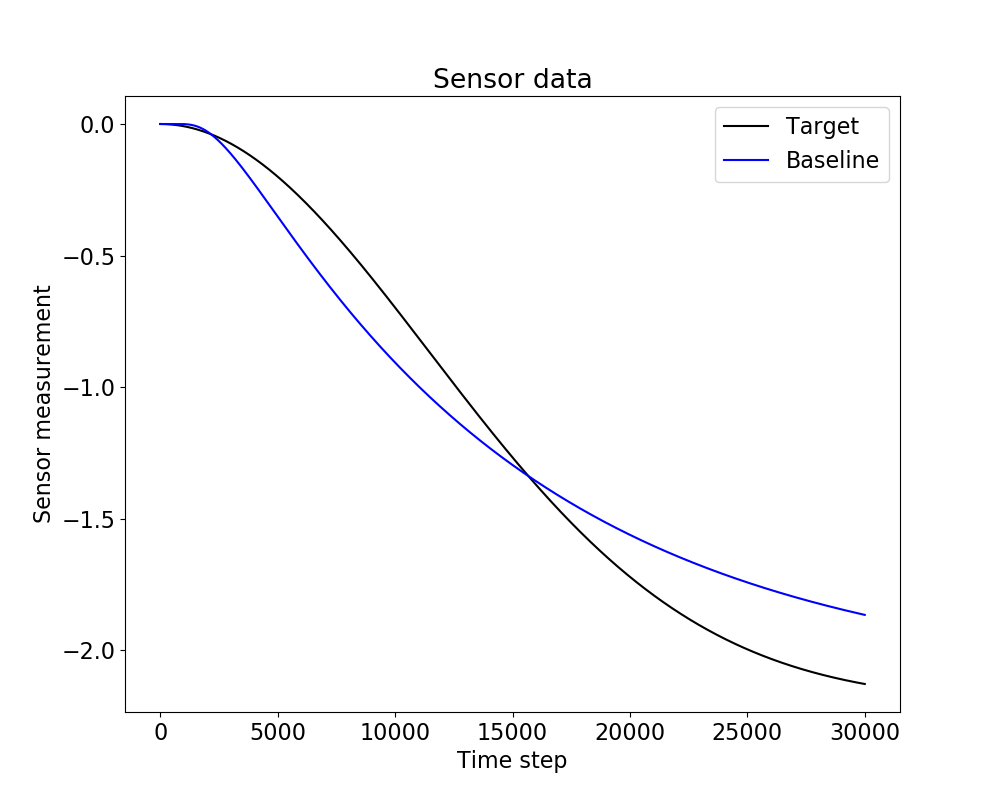
\includegraphics[width=0.6\textwidth]{init_comparison.png}
\caption{Difference in the baseline and target time histories at the sensor location}
\label{res}
\end{figure}

\begin{figure}[H]
\centering
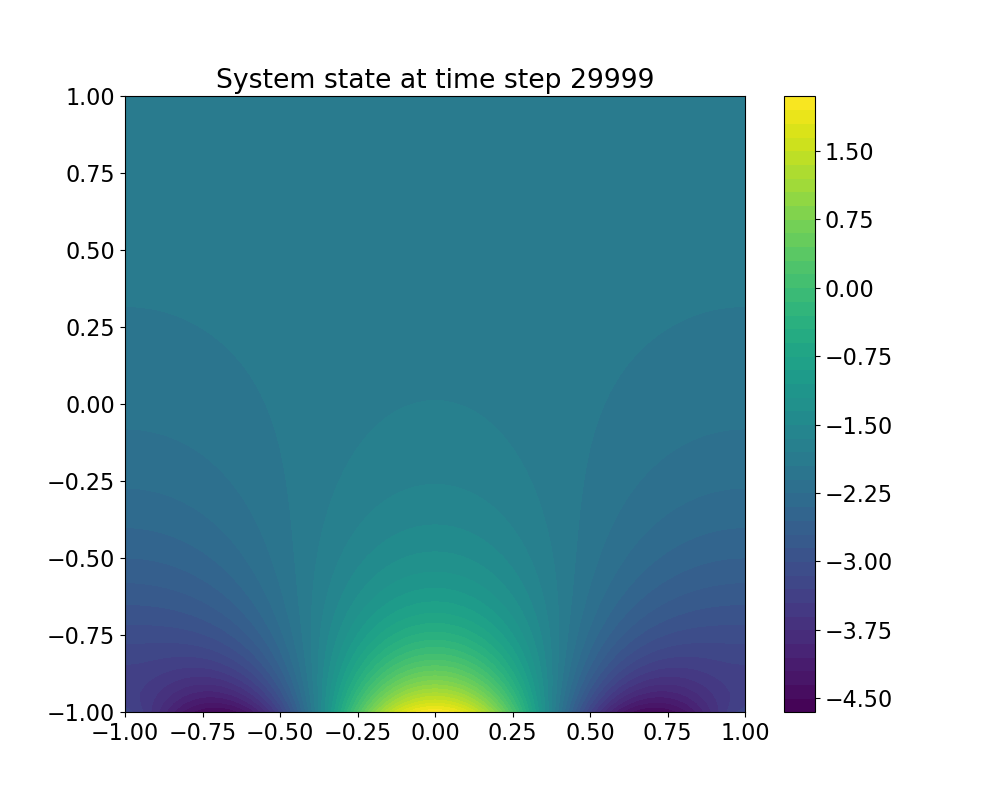
\includegraphics[width=0.6\textwidth]{field.png}
\caption{Baseline state field}
\label{res}
\end{figure}

The optimization reduces the objective function $J$ by more than $2$ orders of magnitude and the corresponding plots have been shown as follows

\begin{figure}[H]
\centering
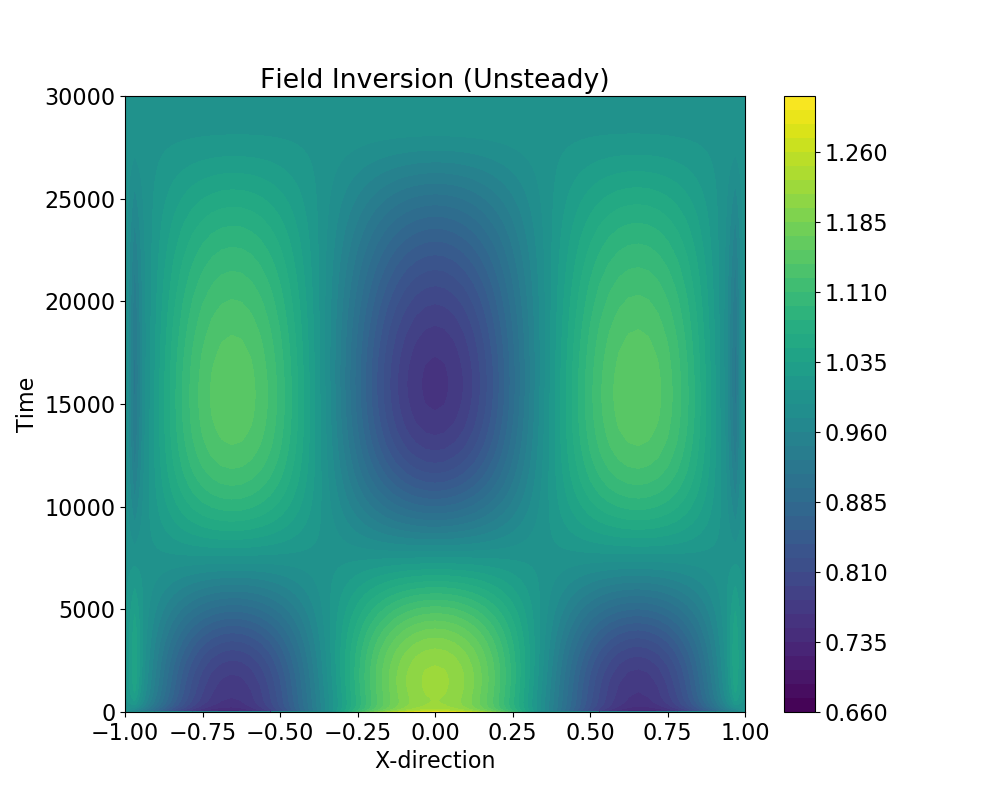
\includegraphics[width=0.6\textwidth]{beta_opt.png}
\caption{Optimal 1-D time varying $\beta$ field}
\label{res}
\end{figure}

\begin{figure}[H]
\centering
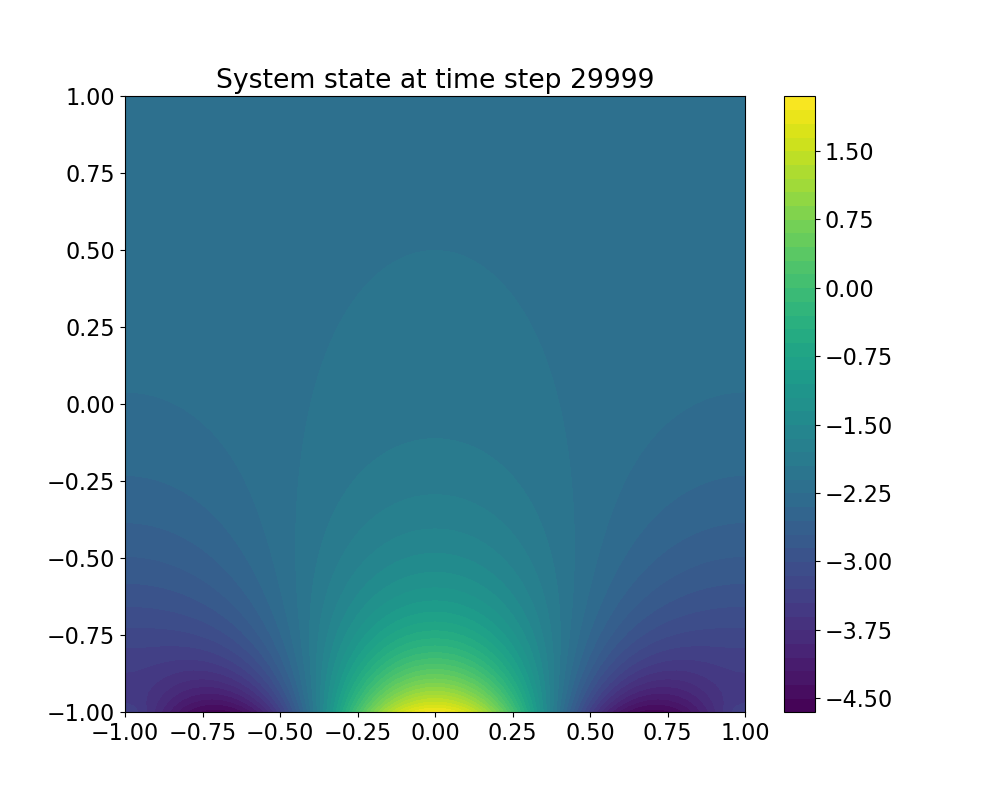
\includegraphics[width=0.6\textwidth]{corrfield.png}
\caption{Corrected state field}
\label{res}
\end{figure}

\begin{figure}[H]
\centering
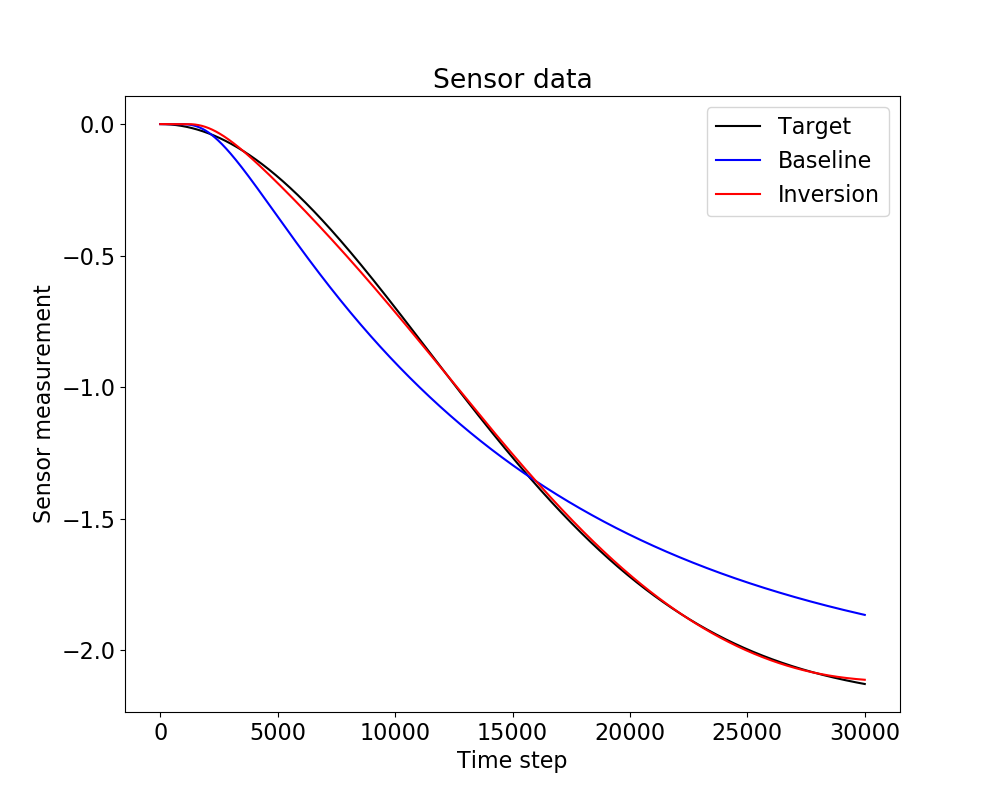
\includegraphics[width=0.6\textwidth]{final_comparison.png}
\caption{Correction in the time history recorded at the sensor location}
\label{res}
\end{figure}
%\eject \pdfpagewidth=8.5in \pdfpageheight=11.5in
%\end{landscape}
%
%================================================================================================================================================================================
%

\end{document}
